\newpage
\section{LITERATURE REVIEW}

\subsection{Human Audio Perception}

The human ear is an exceedingly complex organ.  To make matters even more difficult, the information from two ears is combined in a perplexing neural network,
the human brain. \cite{smith2013}\\
\\
\textit{Figure 1} illustrates the major structures and processes that comprise the human ear. The outer ear is composed of two parts, the visible flap of skin and
cartilage attached to the side of the head, and the ear canal, a tubeabout 0.5 cm in diameter extending about three cm into the head. These structures direct environmental
sounds to the sensitive middle and inner ear organs located safely inside of the skull bones. Stretched across the end of the ear canal is a thin sheet of tissue called the
tympanic membrane or eardrum. Sound waves striking the tympanic membrane cause it to vibrate. The middle ear is a set of small bones that transfer this vibration to the cochlea
(inner ear) where it is converted to neural impulses. The cochlea is a liquid filled tube roughly two mm in diameter and three cm in length.
\begin{figure}[h]
        \centering
        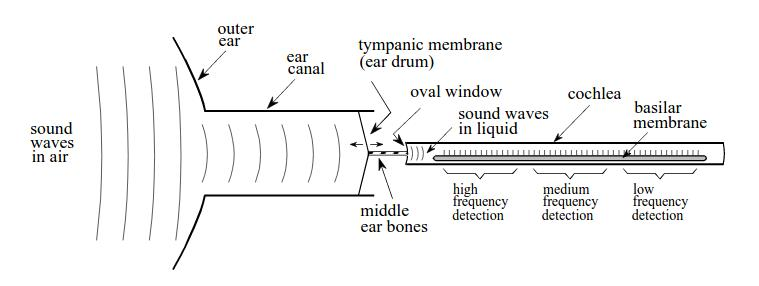
\includegraphics[width=150mm]{resources/humanear.jpg}
        \caption{Functional Diagram of Human Ear}
        \label{fig:figure1}
\end{figure}

Music can be defined as organised sound comprising the following structural elements: pitch, timbre, key, harmony, loudness (or amplitude), rhythm, meter, and tempo. Processing
these elements involves almost every region of the brain and nearly every neural subsystem.\\
\\
Sound does not exist outside of the brain; it is simply air molecules moving. Sound is produced by vibrating air molecules connecting with the
eardrum at varying frequencies (pitch) and velocities (amplitude). The process starts with the brain’s primary auditory cortex receiving a signal from the eardrum/inner ear
which immediately activates our ‘primitive’ brain, the cerebellum. The cerebellum is the oldest part of the brain in evolutionarily terms and plays an important part in motor control.
It contributes to coordination, precision, and accurate timing of movements. The ear and the primitive brain are known collectively as the low-level processing units. They perform the
main feature extraction which allows the brain to start analysing the sounds, breaking down the sensory stimulus into pitch, timbre, spatial location, amplitude, reverberant environment,
tone durations, and onset times of different notes. \\
\\
This data is conducted through neurons in the brain; cells specialized in transmitting information, and the basic building blocks of the nervous system.
The output of these neurons connects to the high-level processing units located in the frontal lobe of the brain. It is important to note that this process
is not linear. The different regions of the brain constantly update each other with new information. \\

\subsection{History of MIR and Music Classification}

The field of Music Information Retrieval (MIR) can be traced back to the 60s with reference to the works done by Kassler in \cite{kassler1966}.
Even Automatic Transcription of Music was attempted as early as the 70s \cite{andel1975}. However, there were two limiting factors that prevented progress in the field at the time.
Firstly, the high computational requirements of the problem domain was simply not available. 
And secondly, other related fields of study such as Digital Signal Processing, Speech Processing, and Machine Learning were also not advanced enough.  
So, the field stalled for the next few decades.\\
\\
In the 1990s, the field regained prominence as computational resources improved greatly and the rise of the internet resulted in massive online music collection. So, there was both an opportunity and demand for MIR systems.
The organization of the first International Symposium on Music Information Retrieval (ISMIR 1) in 2000 highlights this resurgence of interest in the field. 
280 people from 25 different countries participated in ISMIR Conference Malaga 2015.\\
\\
As for the methodologies used, MIR in the 90s was influenced by the field of Text Information Retrieval (IR), techniques for searching and retrieving text documents based on user queries.
So, most of the algorithms were developed based on symbolic representations such as MIDI files \cite{Tzanetakis2002a}. One such method is described in \cite{alghoniemy1999}.\\
\\
However, as mentioned in \cite{byrd2002}, identifying approximate units of meaning in MIR, as done by the majority of text-IR methods (words serve as such units) was not easy.\\
\\
Instead, statistical non-transcriptive approaches for non-speech audio signals started being adopted in the second half on the 90s \cite{Tzanetakis2002a}.
This was probably influenced by progress of such methods in other fields of speech processing. 
For example, in \cite{saunders1996}, the authors reported 98\% accuracy in distinguishing music from speech in commercial radio broadcasts.
This was based on the statistics of the energy contour and the zero-crossing rate.\\
\\
In \cite{wold1996}, the authors introduced similar statistical methods for retrieval and classification of isolated sounds.
Similarly, in \cite{scheirer1997}, an algorithm for music-speech classification based on spectral feature was introduced. 
It was trained using supervised learning. \\
\\
And so, starting in the 2000s, instead of methods attempting note-level transcriptions, researchers focused on direct extraction of information of audio signals using Signal Processing and Machine Learning techniques.\\
\\
Currently, three basic strategies are being applied in MIR: \cite{Casey2008}

\begin{itemize}
        \item \textbf{Based on Conceptual Metadata} - Suited for low-specificity queries.

        \item \textbf{Using High-level Descriptions} - Suited for mid-specificity queries.

        \item \textbf{Using Low-level Signal-based Properties} - Used for all specificities.

\end{itemize}

But still most of the MIR techniques being employed at present use low-level signal features instead of high-level descriptors \cite{Kaminskas2012}.
Thus, there exists a semantic gap between human perception of music and how MIR systems work.

\subsection{Audio Processing}

General Audio signal processing is an engineering field that focuses on the computational methods for intentionally altering sounds, methods that
are used in many musical applications.\\
\\
Particularly speaking, music signal processing may appear to be the junior relation of the large and mature field of speech signal processing,
not least because many techniques and representations originally developed for speech have been applied to music, often with good results. However,
music signals possess specific acoustic and structural characteristics that distinguish them from spoken language or other nonmusical signals. \cite{muller2011}\\
\\
In music the most important qualities of sound are: pitch, duration, loudness, and timbre. Duration and loudness are unidimensional, while pitch and timbre are complex and multidimensional. \cite{dooling2014}

\begin{itemize}
        \item \textbf{Loudness} - Intensity of a tone is the physical correlate that underlies the perception of loudness. Loudness variations play an important role in music, but are less important than pitch variations.

        \item \textbf{Duration} - A composer or performer can alter the pace of a piece so that its apparent (virtual) time is slower or faster than clock time. 

        \item \textbf{Timbre} - Timbre is the subjective code of the sound source or of its meaning. According to the American Standards Association, "Timbre
                is that attribute of auditory senstation of which a listener can judge that two steady-state tones having the same pitch and loudness are dissimilar."

        \item \textbf{Pitch} - Pitch is related to the frequency of a pure tone and to the fundamental frequency of a complex tone. In its musical sense, pitch
                has a range of about 20 to 5000 Hz. Some five to Zseven harmonics of a complex tone can be heard out individually by paying close attention. There
                is a dominance region for pitch perception, roughly from 500 to 2000 or 3000 Hz. Harmonics falling in the dominance region are most influential 
                with regard to pitch.

\end{itemize}

Again, these types of low dimensional features extracted from the acoustical signals are more popular than higher dimensional representations such as
Spectrograms for Classification purposes. \cite{prasad2007}

\subsection{Theoretical Background}
\subsubsection{Features}
\paragraph{Compactness.}
It is the measure of the noisiness of a signal. It is found by comparing the 
components of a window’s magnitude spectrum with the magnitude spectrum of its  
neighbouring windows.\\ 
\\
If M[n], M[n-1] and M[n+1] $>$ 0, then
\begin{equation}
        compactness = \sum_{n=2}^{N-1}{((|20*log(M[n]))-20*(log(M[n-1])+log(M[n])+log(M[]n+1))/3|)}
\end{equation}
otherwise,
\begin{equation}
        compactness = 0
\end{equation}
where M[n] is the Magnitude Spectrum at internal n.

\paragraph{Mel-Frequency Cepstral Coefficients.}
It is a representation of the short-term power spectrum of a sound, based on a linear cosine 
transform of a log power spectrum on a nonlinear mel scale of frequency.\\
\\
\textbf{Algorithm}
\begin{enumerate}[(i)]
        \item \textbf{Framing:}
                The process of segmenting the speech samples obtained from analog to digital conversion(ADC) into a small frame with the length within
                the range of 20 to 40 msec. The voice signal is divided into frames of Nsamples. Adjacent frames are being separated by M(M $<$ N).
        \item \textbf{Hamming Window:}
                Hamming window is used as window shape by considering the next block in feature extraction processing chain and integrates all the 
                closest frequency lines. The Hamming window equation is given as:\\
                \\
                If the window is defines as W(n), 0 $\le$ n $\le$ N-1 where\\
                N = number of samples in each frame\\
                Y[n] = Output signal
                X(n) = Input signal
                W(n) = Hamming window,\\
                then the result of windowing signal is shown below:
                \begin{equation}
                        Y(n) = X(n) \times W(n)
                \end{equation}
                \begin{equation}
                        W(n) = 0.54 - 0.46cos\Big(\frac{2 \pi n}{N-1}\Big), \hspace{10mm}0 \le n \le N-1
                \end{equation}
        \item \textbf{Fast Fourier Transform:}
                To convert each frame of N samples from time domain into frequency domain. The Fourier Transform is to convert the
                convolution of the glottal pulse U[n] and the vocal tract impulse response H[n] in the time domain. This statement supports the equation below:
                \begin{equation}
                        Y(w) = FFT[h(t)*X(t)] = H(w) * X(w)
                \end{equation}
                If X(w), H(w) and Y(w) are the Fourier Transform of X(t), H(t) and Y(t) respectively.
        \item \textbf{Mel Filter Bank Processing:}
                The frequencies range in FFT spectrum is very wide
                and voice signal does not follow the linear scale as shown in figure 2.2 is then
                performed. This figure shows a set of triangular filters that are used to
                compute a weights sum of filter spectral components so that the output of
                process approximates to a Mel scale. Each filter’s magnitude frequency re-
                sponse is triangular in shape and equal to unity at the centre frequency and
                decrease linearly to zero at centre frequency of two adjacent filters [7,8].
                Then, each filter output is the sum of its filtered spectral components. After
                that the following equation is used to compute the Mel for given frequency
                f in Hz:
                \begin{figure}[h!]
                        \centering
                        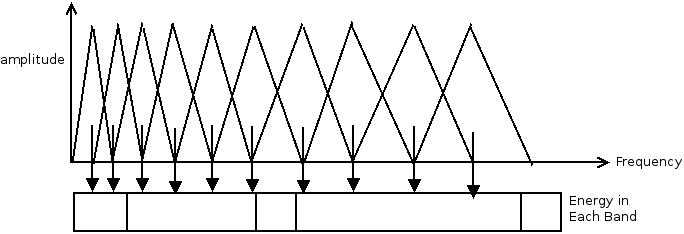
\includegraphics[width=150mm]{resources/melscale}
                        \caption{Mel scale filter bank}
                        \label{fig:Melscale}
                \end{figure}
                This figure shows a set of triangular filters that are used to compute a weights sum of filter spectral components so that the output
                of process approximates to a Mel scale. Each filter's magnitude frequency response is triangular in shape and equal to unity at the
                centre frequency and decrease linearly to zero at centre frequency of two adjacent filters [7,8]. Then, each filter output is the sum of its
                filtered spectral components. After that the following equation is used to compute the Mel for given frequency f in Hz:
                \begin{equation}
                        M(f) = 1125ln\Big(1+\frac{f}{700}\Big)
                \end{equation}
        \item \textbf{Discrete Cosine Transform:}
                This is the process to convert the log Mel spectrum into time domain using Discrete Cosine Transform(DCT). The result of the conversion is
                called Mel Frequency Cepstrum Coefficient. The set of coefficient is called acoustic vectors. Therefore, each input utterance is transformed
                into a sequence of acoustic vector.
\end{enumerate}

\paragraph{Pitch.}
It is a perceptual property of sounds that allows their ordering on a frequency­related scale, or 
more commonly, pitch is the quality that makes it possible to judge sounds as "higher" and "lower" in 
the sense associated with musical melodies.\\  
\\
It is a subjective psychoacoustical attribute of sound, and hence is approximately quantified 
as fundamental frequency.Pitch is an auditory sensation in which a listener assigns musical tones to 
relative positions on a musical scale based primarily on their perception of the frequency of 
vibration.Pitch is closely related to frequency, but the two are not equivalent. Frequency is an 
objective, scientific attribute that can be measured. Pitch is each person's subjective perception  of a 
sound wave, which cannot be directly measured. However, this does not necessarily mean that most 
people won't agree on which notes are higher and lower.\\ 
\\
\textbf{Algorithm}
\begin{enumerate}[(i)]
        \item Model the signal $x_t$ as a periodic function with period T, by definition invariant for a time shift
                of T
                \begin{equation}
                        x_t - x_{t+T} = 0,\hspace{10mm}\forall t
                \end{equation}
                The same is true after taking the square and averaging over a window
                \begin{equation}
                        \sum_{d=t+1}^{t+W}{(x(j)-x(j+\tau))^2} = 0
                \end{equation}
                    Conversely, an unknown period may be found by forming a difference function and searching for 
                    the values of $\tau$ for which the function is zero.
            \item The cumulative mean normalized difference function is calculated by dividing each value of the old 
                    by its average over shorter-lag values. It differs from difference function in the first step in that it 
                    starts at 1 rather than 0, tends to remain large at low lags, and drops below 1 only where the first 
                    difference function falls below average. 
            \item Set an absolute threshold and choose the smallest value of $\tau$ that gives a minimum of the  
                    difference function obtained in the second step deeper than that threshold. If none is found, the 
                    global minimum is chosen instead. With a threshold of 0.1, the error rate drops significantly. 
            \item Each local minimum of the second difference function and its immediate neighbors is fit by a 
                    parabola, and the ordinate of the interpolated minimum is used in the dip-selection process. The 
                    abscissa of the selected minimum then serves as a period estimate. Actually, one finds that the 
                    estimate obtained in this way is slightly biased. To avoid this bias, the abscissa of the corresponding 
                    minimum of the raw difference function(the first) is used instead. 
\end{enumerate}

\paragraph{Tempo.}
The beat is the regularly occurring pattern of rhythmic stresses in music. When we count, tap or clap along 
with music we are experiencing the beat. Try tapping your finger along with different types of music and see 
what happens.\\ 
\\
Tempo is the speed of the beat, usually expressed in Beats Per Minute(BPM). For example, at 120 BPM 
there will be 120 beats in one minute. Tempo can also be expressed verbally with different music terms, 
such as Slowly, Fast, Allegro, or Largo.\\
\\
\textbf{Algorithm}
\begin{enumerate}[(i)]
        \item Parse an audio file into samples, s[n], with a corresponding sampling rate, SR.
        \item Break the audio file into N windows of 1024 samples.
        \item Calculate the FFT of each window.
        \item Calculate the power spectrum(P) of each window form the corresponding FFT results.
        \item Calculate the spectral flux(F) from the power spectrum(P) of each window, i:
                \begin{equation}
                        F_i = (P_i - P_{i-1})^2
                \end{equation}
        \item Find the mean flux, $F_{av}$, across all windows.
        \item Set $F_i$, the flux for each window, to 0 if it is not at least 1.5 times $F_{av}$ (this value
                was experimentally determined). This gives a generous estimation of note onsets.
        \item Use autocorrelation to find the histogram of lag frequencies, L:
                \begin{equation}
                        L[lag] = \sum_{i}^{N}{F[i]F[i+lag]}
                \end{equation}
        \item Calculate the effective sampling rate, $S_{eff}$, found in F and L.
                \begin{equation}
                        SR_{eff} = \frac{SR}{1024}
                \end{equation}
        \item Convert the lag histogram L[lag] into a tempo histogram L[BPM] with bins of beats per
                minute by reversing the order of L and converting the bin lag indices, lag, to BPM:
                \begin{equation}
                        L[BPM] = L\Big(\frac{60*SR_{eff}}{lag}\Big)
                \end{equation}
        \item The result of step (x), L[BPM], is a tempo histogram with bin labels corresponding to beats 
                per minute and bin frequencies correspoding to frequencies of inter-peak intervals.

\end{enumerate}
\paragraph{Root Mean Square.}
The root mean square(abbreviated RMS of rms) is defined as the square root of mean square(the arithmetic mean
of the squares of a set of numbers).
\begin{equation}
        x_{rms} = \sqrt{\frac{1}{n}(x_1^2+x_1^2+...+x_n^2)}
\end{equation}
where there is set of n values \{$x_1, x_2, ......., x_n$\}.

\paragraph{Spectral Centroid.}
The spectral centroid is defined as the center of gravity of the magnitude spectrum of the STFT.
\begin{equation}
        C_t = \frac{\sum\limits_{n=1}^{N}{M_t[n]*n}}{\sum\limits_{n=1}^{N}{M_t[n]}}
\end{equation}
where $M_t[n]$ is the magnitude of the Fourier transform at frame t and frequency bin n.\\
The centroid is a measure of spectral shape and higher centroid values correspond to "brighter" textures with more high frequencies.

\paragraph{Spectral Flux.}
The spectral flux is defined as the squared difference between the normalized magnitudes of successive spectral distributions.
\begin{equation}
        F_t = \sum_{n=1}^{N}{(N_t[n]-N_{t-1}[n])^2}
\end{equation}
where $N_t[n]$ and $N_{t-1}[n]$ are the normalized magnitude of the Fourier transform at the current frame t, and the previous frame t-1, 
respectively.\\ 
The spectral flux is a measure of the amount of local spectral change.

\paragraph{Spectral Roll-off Point.}
The spectral roll-off is defined as the frequency $R_t$ below which 85 per cent of the magnitude distribution is concentrated.
\begin{equation}
        \sum_{n=1}^{R_t}M_t[n] = 0.85*\sum_{n=1}^{N}{M_t[n]}
\end{equation}
The roll-off is another measure of spectral shape.

\paragraph{Spectral Variability.}
  Spectral variability is the standard deviation of the magnitude spectrum. This gives the 
  measure of the variance of a signal's magnitude spectrum. 
  \begin{equation}
          Spectral variability = \sqrt{\frac{1}{N-1}-(\sum_{n=1}^{N}{M[n]-mean})^2}
  \end{equation}
  where M[n] = Magnitude spectrum of the signal at interval n,
  Mean = mean of the magnitude spectrum.

\paragraph{Zero Crossing.}
The zero crossing is defined as the number of times the waveform changed sign.
\begin{equation}
        Z_t = \frac{1}{2}\sum_{n=1}^{N}{|sign(x[n])-sign(x[n-1])|}
\end{equation}
where the sign fucntion is 1 for positive arguments and 0 for negative arguments and\\
x[n] is the time domain signal for frame t.\\
Time domain zero crossings provide a measure of the noisiness of the signal.



\subsubsection{Classifier}
In machine learning and statistics, classification is the problem of identifying to which of a set of categories(sub-populations) a 
new observation belongs, on the basis of a training set of data containing observations(or instances) whose category membership is known.
In the terminology of machine learning, classification is considered an instance of supervised learning where a training set of correctly identified observations is available.
The corresponding unsupervised procedure is known as clustering, and involves grouping data into categories based on some measure of inherent similarity or distance.
An algorithm that implements classification,especially in a concrete implementation, is known as a classifier.\\
\\
A variety of methods have been used for music classification. Some of the popular ones are
SVM, K-means, K-nearest neighbours and variants of Neural Networks.
The results are also widely different. In \cite{Neumayer2004} 61 per cent accuracy has been achieved using
a Multilayer Perceptron based approach while in \cite{Kour2015}, the authors have managed 95 per cent
(for Back Propagation Neural Network) and 83 per cent (for SVM).
In \cite{Koerich2013}, the authors have achieved 71 per cent accuracy using an additional rejection and
verification stage.\\
\\
In \cite{Haggblade2011}, simpler and more naive approaches (k-NN and k-Means); and more sophisticated
neural networks and SVMs have been compared. The author found the latter gave better
performance.\\
\\
However, lots of unique methods – either completely novel or a variation of a standard
method – have been put into use too. In \cite{Nasridinov2014}, the authors propose a method that uses Chord
labeling (ones and zeros) in conjunction with a k-windowSubsequenceMatching algorithm
used to find subsequence in music sequence and a Decision tree for the actual genre classifi-
cation.\\
\\
It is also noted that high-level and contextual concepts can be as important as low-level
content descriptors\cite{Anglade2010}.\\
\\
After these all research, we decided to go with K-means, artificial neural network based on backpropagation
and support vector machine. Artificial neural network and support vector machine were chosen as they appeared to be famous in the field. Our choice for K-means 
was based on the fact that it was simple yet powerful unsupervised procedure.

\paragraph{K-means Clustering.}

K-means is one of the most popular algorithm used for clustering of a given data sets. It is a method of vector quantization, originally
from signal processing, that is popular for cluster analysis in data mining. It aims at partition n obsevations into k clusters in which each observation
belongs to the cluster with the nearest mean, serving as a prototype of the cluster. This results in a partitioning of the data space into Voronoi cells. 
In other words, it clusters all the data points which resemble close
to each other or we can that it cluster all those data points together which have the lowest cost among themselves based on the distance metric.
The problem is computationally difficult(NP-hard); however, there are efficient heuristic algorithms that are commonly employed and converge quickly to a local optimum.
It has loose relationship to the k-nearest neighbor classifier.\\ 
\\
Regarding computational complexity, finding the optimal solution to the k-means clustering problem for obsevations in d dimensions is NP-hard in genral Euclidean space
d even for 2 clusters and NP-hard for a general number of clusters k even in the plane. It k and d (the dimension) are fixed, the problem can be solved in time
$O(n^{dk+1}logn)$, where n is the number of entities to be clustered.
The choice for this algorithm was based on our research and some had already implemented it \cite{Haggblade2011}. Most of the research papers has enlisted this algorithm like in \cite{muller2011}, 
\cite{Hamerly2002}, \cite{Haggblade2011}. So, our reason for implementation of this algorithm was:
\begin{enumerate}[(i)]
        \item Most of the research papers has shown its use in music classification.
        \item It is a pretty straightforward and simple algorithm.
        \item We wanted to have full control over all aspects related to the implementation: the initialization method, distance metric, etc.
\end{enumerate}
The implementation however is basic in the sense that no modification has been done on the algorithm to better suit the problem domain. 
Some finer points of the implementation are discussed below after quickly going over the algorithm itself.\\ 
\\
\textbf{Algorithm}\\
Let X = { $x_1, x_2,.... ,x_n$ be the set of data points and V = { $v_1,v_2 , ...,v_c$ } be the set of centers. 
        \begin{enumerate}[(i)]
                \item Randomly select 'c' cluster centers. 
                \item Calculate the distance between each data point and cluster centers. 
                \item Assign the data point to the cluster center whose distance from the cluster center is minimum of all the cluster centers. 
                \item Recalculate the new cluster center: 
                        \begin{equation}
                                v_i=\frac{1}{c_i}\sum_{j=1}^{c_i}{x_i}
                        \end{equation}
                \item  Recalculate the distance between each data point and new obtained cluster centers. 
                \item If no data point was reassigned then stop, otherwise repeat from step 3).
        \end{enumerate}
\textbf{Initialization method}\\
Commonly used initialization methods are Forgy and Random Partition. The Forgy method randomly chooses k observations from the data set and uses
these as the initial means. The Random Partition method first randomly assigns a cluster to each observation and then proceeds to the update step, thus
computing the initial mean to be the centroid of the cluster’s randomly assigned points. The Forgy method tends to spread the initial means out, while
Random Partition places all of them close to the center of the data set. According to \cite{Kour2015}, the Random Partition method is generally preferable for
algorithms such as the k-harmonic means and fuzzy k-means. For expectation maximization and standard k-means algorithms, the Forgy method of initialization is preferable.\\
\\
And with these facts in mind, we went for the random initialization method. This method has been used in \cite{muller2011} too although they have also added
the constraint that the centroids be separated by at least a threshold KL-divergence distance. As the choice of initial centroids have a drastic
effect on the cluster formed, we have also considered other methods of initialization such as the breakup method which uses the actual data points
and the scrambled midpoints method which uses synthetic data points as suggested in \cite{prasad2007}. So after our research on this, we found that 
scrambled midpoints to be much more efficient and lead to better clustering. So based on \cite{Apon2006}, scrambled midpoints technique was
chosen for initialization.\\
\\ 
In scrambled midpoints initialization method, at first our whole data range or in our case each feature range was broken down into k-paritions which were
all equal. Then midpoints were taken of those equal partitions for each feature partition range. Provided there are n-features with k
number of clusters needed, then we have n*k different possibilities. Now all these midpoints of each range of n-features were scrambled among
each other to form k different initialization points/vectors representing all those n-features. It should be clear that there is no repetition of the midpoint of same range 
of same feature during scrambling of midpoints to form initialization points/vectors.\\  
\\
\textbf{Distance Metric}\\
Apart from the initialization method, K-means is also highly sensitive to the distance metric used. There are many distance metric but most popular ones are: 
\begin{itemize}
        \item Manhattan distance
        \item Euclidean distance
        \item Minkowski distance
\end{itemize}
Most of the times, K-Means is implicitly based on pairwise Euclidean distances between points, because the sum of squared deviations from centroid (that it tries to minimize) is equal
to the sum of pairwise squared Euclidean distances divided by the number of points \cite{Neumayer2004}.\\ 
\\
As such, we decided to use Euclidean distance with weights for the three different features added to give us a way to control the metric. Thus, the
distance between two songs S1 and S2 is given by: 
\begin{equation}
        Distance(d)=\sqrt[2]{w_I(I_1-I_2)^2+w_M\sum_{i}{(M_{1i}-M_{2i})^2}+w_R\sum_{i}{(R_{1j}-R_{2j})^2}}
\end{equation}
Where: $w_I$ , $w_M$  and $w_R$ are the weights for Intensity, MFCC and Rhythm respectively. 

\paragraph{Artificial Neural Network.}
In machine learning and cognitive science, an artificial neural networks(ANN) is a network inspired by biological neural networks(the central nervous systems of 
animals, in particular the brain) which are used to estimate or approxiamte functions that can depend on a large numbers of inputs that are generally unknown.
Our research shows whether the research is related to our field or other, most of the time for machine learning researchers used artificial neural network.
So our choice was simple as it was based on supervised learning and comparatively simple than other complicated unsupervised learning.
Research papers \cite{Koerich2013}, \cite{Neumayer2004}, ,\cite{Anglade2010}, \cite{Haggblade2011} and \cite{Kour2015} shows the implementation of artificial neural network in the field of
music classification.\\
\\
Artificial neural networks are typically specified using three things:
\begin{itemize}
        \item \textbf{Architecture:} 
                It specifies what variables are involved in the network and their topological relationships- for example the variable involved
                in a neural network might be the weights of the connections between the neurons, along with activities of the neurons. In an artificial
                neural network, there are one or more hidden layers in between input and output layers with all the neurons connecting to each other.
        \item \textbf{Activity Rule:}
                Most neural network models have short tiem-scale dynamic: local rules define how the activities of the neurons change in reponse to each other.
                Typically the activity rule depends on the weights(the parameters) in the network.Here in our case, the set of input neuronse
                is activated by the feature values like MFCC, pitch,etc. There activation function present to trigger the respective neuron. Most of the time
                activation function are non linear, differential mathematical functions like sigmoid, hyperbolic tangent, etc.
        \item \textbf{Learning Rule:}
                The learning rule specifies the way in which the neural network's weights change with time as the learning takes progress. This learning is usually viewed as 
                taking place on a longer time place than time scale of the dynamicx under the activity rule. Usually the learning rule will depend on the activites of the 
                neurons. In our case the learning depends on the values of the target values supplied by a teacher and on the current value of the weights.
\end{itemize}

\begin{figure}[h]
        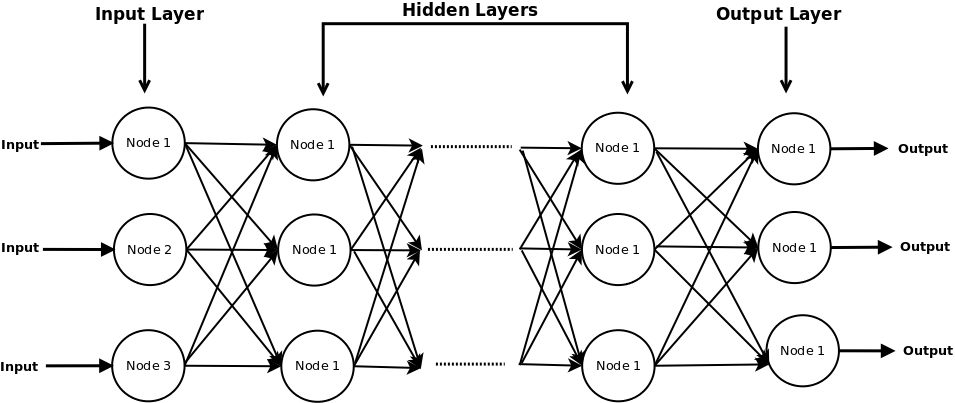
\includegraphics[width=150mm]{resources/ann}
        \caption{General structure of artificial neural network}
\end{figure}
For a system, generally the architecture is created as per the need. Generally for that there is lot of trial and error methodology involved
to determine the correct number of hidden layers and neurons needed. In most cases, one hidden layer is suffiecient for the system but if 
the nature of system or data is perplexing then in accordance to expected result and current behavior, number of hidden layers of nodes can be increased.\\
\\
The concept of cost function is an important in context of artificial neural network. It measures how far away a particular solution is from an
optimal solution. We can also say that the cost of the optimal solution is minimum. So, the target of our artifical neural network is to
try to meet the cost of optimal solution. While it is possible to define some arbitrary ad hoc cost fucntion, frequently a particular cost will be used, either
because it has desirable properties (such as convexity) or because it arises naturally from a particular formulation of problem. Ultimately, the cost
fucntion will depend on the desired task. One of the mostly used cost function is squared error measure between the output value O and the target value t.
\begin{equation}
        E = (t-y)^2
\end{equation}
where E is the discrepancy or error.\\
\\
Using this cost, the neural network tries to adjust it weights in order to minimize the cost function. This exact process is called learning.
Supervised learning, unsupervised learning and reinforcement learning are the three major paradigms of learning. We are opting for the supervised learning.
The reason for this choice is that unsupervised learning and reinforcement learning are comparatively more complex and also supervised learning have been doing 
great job in this music classification field based on research papers \cite{Neumayer2004}, \cite{Haggblade2011}, \cite{Kour2015}. Supervised learning 
requires the correct class label to be provided along with the training dataset for the neural network so that it can adjust it's weight based on the cost function 
of incorrect/correct class prediction. Backpropagation algorithm is the most popular learning algorithm for neural network out there. The reason for
its popularity might be its simplicity in terms of concept and wide applicability. It's also based on supervised learning. When one tries to minimize cost function
using gradient descent for the class of neural networks called multilayer perceptrons(MLP), one obtains the common and well-known backpropagation algorithm for training neural networks.\\
\\
Backpropagation is a common method of training artificial neural networks used in conjunction with an optimization method such as gradient descent. The 
method calculates the gradient of a loss function with respect to all the weights in the network. The gradient is fed to the optimization method wihich in turn uses it to
update the weights, in an attempt to minimize the loss function. It is a generalization of delta rule to multi-layered feedforward networks, made possible
by using the chain rule to iteratively compute gradients for each layer. Requirements of backpropagation mehod are:
\begin{itemize}
        \item It requires a known, desired output for each input value in order to calculate the loss function gradient.
        \item It requires the activation function used by the artificial neurons/nodes to be differentiable.
\end{itemize}
\textbf{Algorithm}
\begin{enumerate}[(i)]
        \item Run the network forward with your input data to get the network output.
        \item For each output node compute
                \begin{equation}
                        \delta_k = O_k(1 - O_k)(O_k - t_k)
                \end{equation}
        \item For each hidden node calculate
                \begin{equation}
                        \delta_j = O_k(1 - O_k) \sum_{k \in K}{\delta_kW_{jk}}
                \end{equation}
        \item Update the weights and biases as follows:\\
                Given
                \begin{equation}
                        W = -\eta \delta_l O_{l-1}
                \end{equation}
                \begin{equation}
                        \Delta \theta = -\eta \delta_l
                \end{equation}
                apply
                \begin{equation}
                        W + \Delta W \to W
                \end{equation}
                \begin{equation}
                        \theta + \Delta\theta \to \theta
                \end{equation}
\end{enumerate}
where i, j and k represents the input layer, hidden layer and ouput layer respectively,\\
O is the output of a neuron/node,\\
t is the target value,\\
K is the total number of output neurons/nodes,\\
$\Delta$ represent the difference,\\
l denotes every layer.\\
\\
$\eta$ is the learning rate which is defined as the ratio(percentage) that influences the speed and quality of learning.The greater the ratio, the faster the neuron trains;
the lower the ratio, the more accurate the training is. $\theta$ is the bias term which is involved in adjusting the shifting of activation function. The sign of the gradient
of a weight indicates where the error is increasing, this is why the weight must be updated in the opposite direction. The algorithm above is
repeated until performance of the network is satisfactory.

\paragraph{Support Vector Machine.}

In machine learning, support vector machines (SVM) are supervised learning models with 
associated learning algorithms that analyze data used for classification analysis.They are new statistical learning technique that can be seen as a new method for training
classifiers based on polynomial functions, radial basis functions, neural networks, splines or other functions. The popularity of Support Vector machine is huge as lot of researcher papers
\cite{Koerich2013}, \cite{Anglade2010}, \cite{Haggblade2011}, \cite{Kour2015} shows its implementation. Not only in the field of music classification but also on various artificial intelligence field like handwriting
recognition, biological and other sciences. It was also able to overthrow general neural network until the advent of deep learning.\\
\\
The basic support vector machine (SVM) is a binary linear classifier which chooses the hyperplane that represents the largest separation, or margin, between the two classes. So  Support vector machines use
a hyperplane to create a classifier. If such a hyperplane exists, it is known as the maximum­margin hyperplane and the linear classifier it defines is known as a maximum margin classifier. 
If there exists no hyperplane that can perfectly split the positive and negative instances, the soft 
margin method will choose a hyperplane that splits the instances as cleanly as possible, while still 
maximizing the distance to the nearest cleanly split instances. For problems that cannot be linearly separated in the input space, this machine offers a possibility to find a solution by making 
a non-linear transformation of the original input space into a high dimension feature space where an optimal separating hyper plane can be found. Those separating planes are optimal, which means
that a maximal margin classifier with respect to the training data set can be obtained. It is developed by Vladimir Vapnik and co-workers at AT\&T Bell Laboratories in 1995.\\
\begin{figure}[h]
        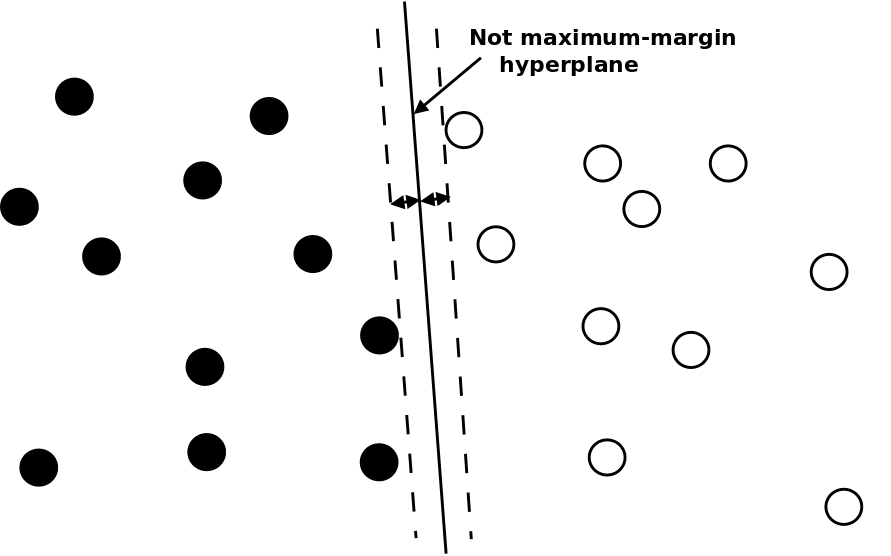
\includegraphics[width=150mm]{resources/misleadinghyperplane}
        \caption{Misleading hyperplane}
\end{figure}
\begin{figure}[h]
        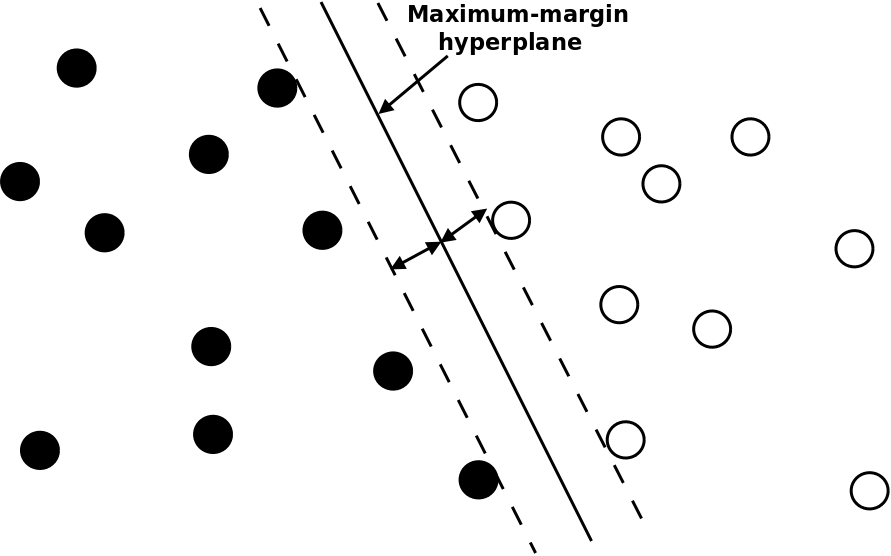
\includegraphics[width=150mm]{resources/svm}
        \caption{Support vector machine with maximum-margin hyperplane}
\end{figure}
The nonlinear SVMs are created by applying the kernel trick to maximum­margin hyperplanes. 
The resulting algorithm is formally similar, except that every dot product is replaced by a nonlinear kernel 
function.\\
\\
\textbf{Kernel Function}\\
The simplest way to divide two groups is with a straight line, flat plane or an N-dimensional hyper plane.
But what if the points are separated by a non-linear region. In such case we would need a non-linear dividing line. Rather than fitting
non-linear curves to the data, support vector machine handles this by using a kernel function to map the data into a different space where
a hyperplane can be used to do the separation. \cite{Anglade2010} shows the use of second order polynomial kernel in the support vector machine.
So, kernel function allows the algorithm to fit the maximum­margin hyperplane in a transformed
feature space. The transformation may be nonlinear and the transformed space be high dimensional. For example, the 
feature space corresponding to Gaussian kernel is a Hilbert space of infinite dimension. Thus though the 
classifier is a hyperplane in the high dimensional feature space, it may be nonlinear in the original input 
space. Maximum margin classifiers are well regularized, so the infinite dimension does not spoil the 
result as the separation will be performed even with very complex boundaries.\\

\begin{figure}[h]
        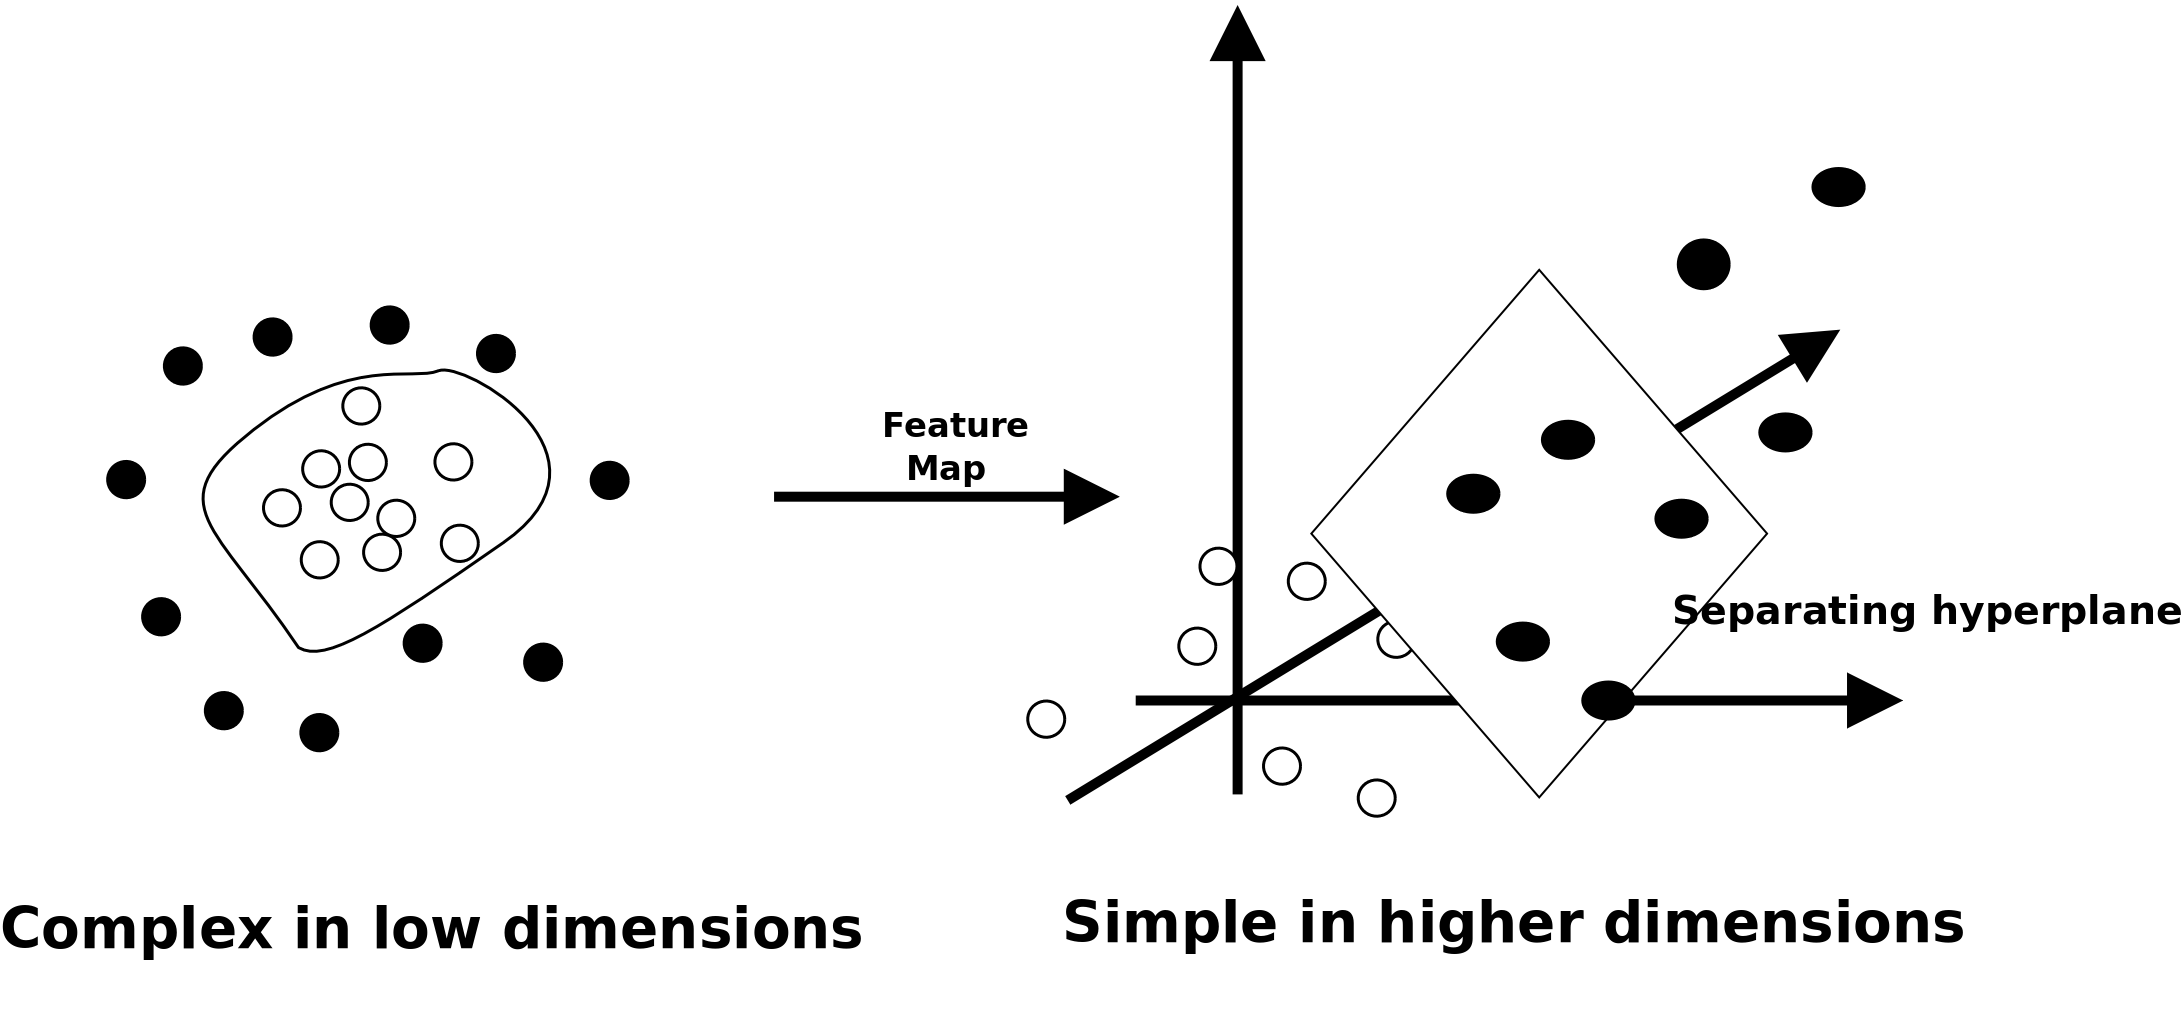
\includegraphics[width=150mm]{resources/kernel}
        \caption{Support vector machine with kernel function}
\end{figure}
\vspace{15mm}
The effectiveness of SVM depends on the selection of kernel, the kernel’s parameters, and soft 
margin parameter c. Given a kernel, best combination of c and kernel’s parameters is often selected by a 
grid­search with cross validation. 
The dominant approach for creating multiclass SVMs is to reduce multi­class problem into 
multiple binary classification problems. Common methods for such reduction is to build binary classifiers 
which distinguish between (i) one of the labels to the rest (one­versus­all) or (ii) between every pair of 
classes (one­versus­one). Classification of new instances for one­versus­all case is done by a 
winner­takes­all strategy, in which the classifier with the highest output function assigns the class. For the 
one ­versus­one approach, classification is done by a max­wins voting strategy, in which every classifier 
assigns the instance to one of the two classes, then the vote for the assigned class is increased by one vote, 
and finally the class with most votes determines the instance classification. To tackle the same multiclass problem \cite{Haggblade2011} has the  
utilization of DAG(Directed Acyclic Graph) SVMs in which a directed acyclic graph(DAG) of two-class SVMs is trained on each pair of classes in the data set.

\subsection{Testing and Validation}
While building a software product, the concept of testing and validation plays an important role throughout its development.
Along with the development of a software product, numerous testing and validation are need to be performed regulary.
In fact, most of the development period is given to testing and validation. It's important as it conforms to whether we are building
product right and whether we are building the right product. After series of testing and validation only we can point that the system
conforms to the desired specifications and need.\\
\\
Since our software project is also research oriented, so we need series of rigorous testing. Not only this, being a predictive system/model
a type of validation and measure for performance is a must, so that it can analyze the result and decide how to progress further accounting the fact.
For our system, we chose cross-validation after we confronted it's popularity for a predictive model and ease of use. Similarly for measure of performance we chose recall, presicion 
and F-measure.\\

\subsubsection{Cross-validation}
Cross-validation is a technique for estimating the performance of a predictive model.
Cross-validation, sometimes called rotation estimation is a model validation technique for assessing how the
results of a statistical analysis will generalize to an independent data set. In a predictive problem like our project, a model is usually given a dataset of known data(training dataset) on which 
the model is trained, and a dataset of unknown data (or first seen data) against which the model is tested (testing dataset). The goal of cross validation is to define a dataset
to "test" the model in the training phase(validation dataset), in order to limit problems like overfitting, give an insight on how the model will generalize to an independent dataset(and unknown dataset, for instance from 
a real problem),etc.\\
\\
One of the main reasons for using cross-validation instead of using the conventional validation is that there is not enough data available to partition it into separate training and test sets without losing
significant modelling or testing capability. There are several cross-validation method out there like leave-p-out cross-validation, leave-one-out cross validation,2-fold cross validaiton, repeated random 
sub-sampling validation, etc. But we decide to got with k-fold cross validation. The main reason for this selection is that k-fold cross-validation estimator can prove to have a lower variance than a single hold-out set 
estimator if the amount of data available is limited. Our main goal with k-fold cross validation is to estimate the expected level of fit of a model to a dataset that is independent of the data that were
used to train the model.\\
\\
In k-fold cross-validation, the original sample is randomly partitioned into k equal sized subsamples. Of the k subsamples,
a single subsample is retained as the validation data for testing the model, and the remaining k − 1 subsamples are used as training
data. The cross-validation process is then repeated k times (the folds), with each of the k subsamples used exactly once as the validation data. The k results from the
folds can then be averaged to produce a single estimation. The advantage of this method over repeated random sub-sampling (see below) is that all
observations are used for both training and validation, and each observation is used for validation exactly once. ten-fold cross-validation is currently
applied in our system. Our music data set is first divided into ten equal samples of songs, and on every run for ten times, a different sample of songs are used for
testing and the rest for training.\\
\\
This k-fold validation validation process is applied with each performance metrics and the appropriate features are taken to classify in our system.

\subsubsection{Measure of Performance}
In a predictive problem, we always need a measure of performance for that predictive model along with cross validation. Based on the value of different attributes falling under 
the measure of performance, we can then have the knowledge of how well the system is performing. It is important because as a matter of fact it provides much deeper insight of the performance of
the predictive model, not only accuracy.\\
\\
Our measure of performance include precision, recall and F-measure. We can say our measure of performance are based on the relevant and non-relevent documents. In this case,
relevant documents are those one which simply belong to the relevant category. Relevant category is also called the true positives. True positive is the number of items correctly
labeled as belong to the positive class or say which are predicted correctly. The not relevant documents are those one which simply are not relevant to the category or say they are false negative. 
False negative is the number of negative items which are predicted to fall under the positive class. False Positive is the number of negative items which are predicted to be in true class.
Similarly, true negative is the number of negative items which are correctly predicted to fall under negative class.

\begin{itemize}
        \item \textbf{Precision}\\
                The precision of a measurement system, related to reproducibility and repeatability, is the degree to which repeated measurements under unchanged
                conditions show the same results. In a classification task, the precision for a class is the number of true positives divided by the total number of elements labeled as 
                belonging to the positive class. A perfect precision score of 1.0 means that every result retrieved by a search was relevant which means falling to the specified class.
                But precision does not say whether all items of that class were correctly predicted.
                \begin{equation}
                        Precision = \frac{True Positive}{True Positive + False Positive}
                \end{equation}
        \item \textbf{Recall}\\
                Recall literally is how many of the true positives were recalled (found), i.e. how many of the correct hits were also found. Recall is also sometimes called sensitivity or probability of detection.
                It is the true positive rate as it measure the proportion of positives that are correctly identified as such. Recall is the number of true positives divided by the total number of elements
                that actually belong to the positive class. A perfect recall score of 1.0 means that all relevant documents were retrieved by search. We can also say that perfect recall shows that all items of a
                class were labeled fall under same class. But recall does not say that how many other items were misclassified to fall under same class.
                \begin{equation}
                        Recall = \frac{True Positive}{True Positive + False Negative}
                \end{equation}
        \item \textbf{F measure}
               A measure that combines precision and recall is the harmonic mean of precision and recall. 
                F measure is the weighted harmonic mean of its the precision and recall of a system. It is sometimes called as balanced F-score. This measure is approximately the average of the two when they are close, and is more generally
                the harmonic mean which for the case of two numbers coincides with the square of the geometric mean divided by the arithmetic mean. There are several reasons that the F-score can be criticized in particular 
                circumstances due to its bias as an evaluation metric. This is also known as the $F_1$ measure, because recall and precision are evenly weighted.
                \begin{equation}
                        F = 2*\frac{Precision*Recall}{Precision+Recall}
                \end{equation}
        \end{itemize}
        All three performance metrics have been used to determine the best features to be used for classification in cases of genre, arousal and valence.\\ 
        \\
    As depicted in the result and analysis section, we can see that not all the features are suitable for the classification. Some features such as intensity or pitch do not contribute 
    the classification but some features such as Mel Frequency Cepstral Coefficients(MFCC) contribute greatly to the classifier’s performance. 



\subsection{Related Works}
    \subsubsection{Genre Based Classification}

\paragraph{Overview.}
Automatic Music Genre Classification (AMGC) is one of the tasks focused by MIR. However, it is not a straightforward one.\\
\\
In \cite{Scaringella2006}, Scaringella et al. discuss how and why musical genres are a poorly defined concept making the task of automatic classification non-trivial.
Still, although the boundaries between genres are fuzzy and there are no well-defined definitions, it is still one of the widely used method of classification of music. 
If we look at human capability in genre classification, Perrot et al \cite{Perrot1999} found that people classified songs--in a ten-way classification setup--with an accuracy of 70\% after listening to 3s excerpts.

\paragraph{Features.}
The features used for genre based classification have been heavily influenced by the related field of speech recognition. 
For instance, Mel-frequency Cepstral Coefficients (MFCC), a set of perceptually motivated features that is widely used in music classification, was first used in speech recognition.\\
\\
The seminal paper on musical genre classification by Tzanetakis et al. \cite{Tzanetakis2002} presented three feature sets for representing timbral texture, rhythmic content and pitch content. 
With the proposed feature set, they achieved a classification accuracy of 61\% for ten musical genre.\\
\\
Timbral features are usually calculated for every short-time frame of sound based on the Short Time Fourier Transform (STFT). 
So, these are low-level features. 
Typical examples are Spectral Centroid, Spectral Rolloff, Spectral Flux, Energy, Zero Crossings, and the afore-mentioned Mel-Frequency Cepstral Coefficients (MFCCs).
Among these, MFCC is the most widely preferred feature \cite{Lippens2004}\cite{Kour2015}. Logan \cite{Logan2000} investigated the applicability of MFCCs to music modeling and found it to be "at least not harmful".\\
\\
Rhythmic features capture the recurring pattern of tension and release in music while pitch is the perceived fundamental frequency of the sound. 
These are usually termed as mid-level features.\\
\\
Apart from these, many non-standard features have been proposed in the literature. \\
\\
Li et al.\cite{Li2003} proposed a new set of features based on Daubechies Wavelet Coefficient Histograms (DWCH), and also presented a comparative study with the features included in the MARSYAS framework.
They showed that it significantly increased the accuracy of the classifier.\\
\\
Anglade, Amélie, et al.\cite{Anglade2010} propose the use of Harmony as a high-level descriptor of music, focusing on the structure, progression, and relation of chords.\\
\\

\paragraph{Classifer.}

A variety of methods have been used for music classification. Some of the popular ones are SVM, K Nearest Neighbours and variants of Neural Networks.
The results are also widely different. In \cite{Neumayer2004}, 61 per cent accuracy has been achieved using a Multilayer Perceptron based approach. 
While in \cite{Koerich2013}, the authors have achieved 71 per cent accuracy through the use of an additional rejection and verification stage.
Haggblade et al. \cite{Haggblade2011}, compared simpler and more naive approaches (k-NN and k-Means) with more sophisticated neural networks and SVMs. 
They found that the latter gave better results.\\
\\
Standard statistical pattern recognition classifiers are also used for AMGC.
They may be simple Gaussian Classifiers or Gaussian mixture model (GMM) classifier, where each class pdf is assumed to consist of a mixture of a specific number of multidimensional Gaussian distributions.
In such an approach, the parameters of each Gaussian component and the mixture weights are estimated using the iterative EM algorithm.\\
\\
However, lots of unique methods -- either completely novel or a variation of a standard method -- have been put into use too. In \cite{Nasridinov2014}, the authors
propose a method that uses Chord labeling (ones and zeros) in conjunction with a k-windowSubsequenceMatching algorithm used to find subsequence in music sequence
and a Decision tree for the actual genre classification.\\
\\
It is also noted that high-level and contextual concepts can be as important as low-level content descriptors. \cite{Anglade2010} 

\subsubsection{Mood Based Classification}

\paragraph{Overview.}

As mood is a very human thing, Mood Based Classification, also known as Mood Emotion Recognition (MER), requires knowledge of both technical aspects as well as the human emotional system.
So, the conceptualization of emotion and understanding of the associated emotion taxonomy is vital. However, it is a difficult thing to do, because 
\begin{enumerate}[(i)]
        \item It is subjective and 

        \item We cannot agree on a model to depict emotional states.
        \end{enumerate}

Usually, two approaces to emotion conceptualization are taken: 

\begin{itemize}
    \item \textbf{Categorical Conceptualization} - This approach to MER categorizes emotions into a number of distinct classes. 
        It requires the belief of base emotions (happiness, anger, sadness, etc) from which all other secondary emotion classes can be derived.\cite{Ekman1992}
        However, the major drawback of the categorical approach is that the number of primary emotion classes is too small in comparison with the richness of music emotion perceived by humans.

    \item \textbf{Dimensional Conceptualization} - It defines Musical Values as numerical values over a number of emotion dimensions. 
        So, the focus is on distinguishing emotions based on their position on a predefined space.
        Most of these conceptualizations map to three axes of emotions: valence (pleasantness), arousal (activation) and potency (dominance).
        By placing emotions on a continuum instead of trying to label them as discrete, this approach can encompass a wide variety of general emotions.

\end{itemize}

\paragraph{Circumplex and Thayer Mood Model.}

One of the Dimensional conceptualization was proposed by Russell (1980) \cite{Russell1980}.
As shown in \textit{Figure 2}, the model consists of a two-dimensional structure involving the dimensions of valence and arousal. 
General emotions are placed within thic circular framework.

\begin{figure}[hlvt!]
        \centering
        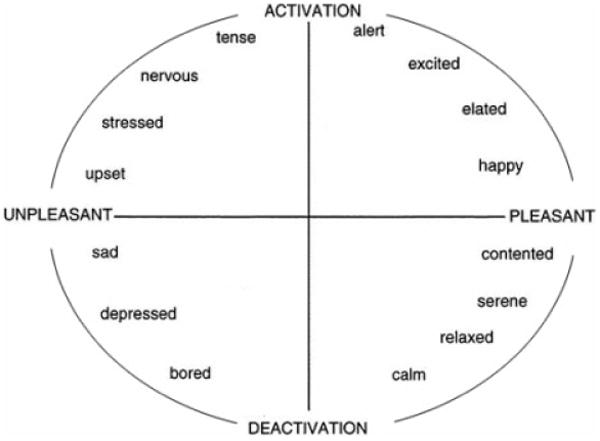
\includegraphics[width=120mm]{resources/circumplex.jpg}
        \caption{A graphical representation of the circumplex model of affect with the horizontal axis representing the valence dimension and the vertical axis representing the arousal or activation dimension.}
        \label{fig:figure2}
\end{figure}

As shown in \textit{Figure 3}, Thayer \cite{Thayer1990} proposed a similar two-dimensional approach that adopts the theory that mood is entailed from two factors: -Stress (happy/anxious) -Energy (calm/ energetic). 
This divides music mood into four clusters: Contentment, Depression, Exuberance and Anxious/Frantic.\\
\\
Although, the two-dimensional approach has been criticized as deficient (leading to a proposal of the third dimension of potency), it seems to offer the right balance between sufficient "verbosity" and low complexity \cite{Juslin2001}.

\begin{figure}[hlvt!]
        \centering
        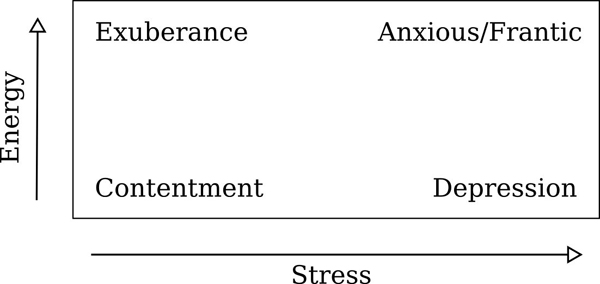
\includegraphics[width=120mm]{resources/thayerModel.jpg}
        \caption{Thayer's two-dimensional model of mood}
        \label{fig:figure3}
\end{figure}

\paragraph{Features.}

Some of the commonly used features in MER are:

\begin{itemize}
    \item \textbf{Energy}: Energy related features such as audio power, loudness, specific loudness sensation coefficients (SONE), are correlated to the perception of arousal. 
        Lu et al. \cite{Lu2006} used it to classify arousal.

    \item \textbf{Rhythm}: Flowing/fluent rhythm is associated with positive valence while firm rhythms with negative valence.

    \item \textbf{Melody}: These include features such as Pitch (perceived fundamental frequency), chromogram centroid, etc.

    \item \textbf{Timbre}: As with the AMGC problem, MFCC is widely used in MER too. Apart from MFCC, octave-based spectral contrast as well as DWCH (Daubechies wavelets coefficient histogram) are also proposed in literature.
        
\end{itemize}

So, we see that the features used in MER are almost the same as those in AMGC. However, Fu et al. note in their extensive survey on Audio-based Music Classification \cite{Fu2011} that although their effectiveness is debatable, mid-level features such as Rhythm seem to be more popular in MER.


\paragraph{Classifiers.}

The algorithms used in AMGC are also popular in MER. So, support vector machines, Gaussian mixture models, neural networks, and k-nearest neighbor are the ones regularly used.

